\section{Setup of test environment for PostgreSQL experiments}

\subsection{Creating test environment for PostgreSQL}\label{pg_setup}
The PostgreSQL instance was 

The Powershell script below is the template for our test environment on the Azure Database for PostgreSQL Single Server.

%A$ecurePassw000rd
\begin{verbatim}
    $Password = Read-Host -Prompt 'Please enter your password' -AsSecureString
    $RGName = "myresourcegroup"
    
    az group create --name $RGName --location northeurope
    
    New-AzPostgreSqlServer `
        -Name bachelorgroup119postgrestest1 `
        -ResourceGroupName $RGName `
        -Sku GP_Gen5_2 `
        -GeoRedundantBackup Enabled `
        -Location northeurope `
        -AdministratorUsername myadmin `
        -AdministratorLoginPassword $Password
\end{verbatim}

\subsection{Data population} \label{pg_populate}
The script below was used to populate the database. 
\begin{minted}[breaklines=true,breakanywhere=true]{python}
import psycopg2
# Connection string information
host = "bachelor119-performance.postgres.database.azure.com"
dbname = "postgres"
user = "bachelor119@bachelor119-performance"
password = "performance-test1"
sslmode = "require"
# Connection string constructed
conn_string = "host={0} user={1} dbname={2} password={3} sslmode={4}".format(host, user, dbname, password, sslmode)
conn = psycopg2.connect(conn_string) 
cursor = conn.cursor()
# Check for duplicate tables
cursor.execute("DROP TABLE IF EXISTS inventory;")
# Create table
cursor.execute("CREATE TABLE inventory (id serial PRIMARY KEY, one BIGINT, two BIGINT, three BIGINT);")
# Insert some data into the table
cursor.execute("INSERT INTO inventory (one, two, three) SELECT generate_series(1, 90000000), generate_series(1, 90000000), generate_series(1, 90000000);")
# Resolve connection
conn.commit()
cursor.close()
conn.close()
\end{minted}

\subsection{Postgres: Azure backup setup}
\label{pg_azurebackup}

In order to back up a postgres server with Azure Backup the first step is to click the "Backup"-option on top of the "Backup instances"-blade inside the Backup Vault.
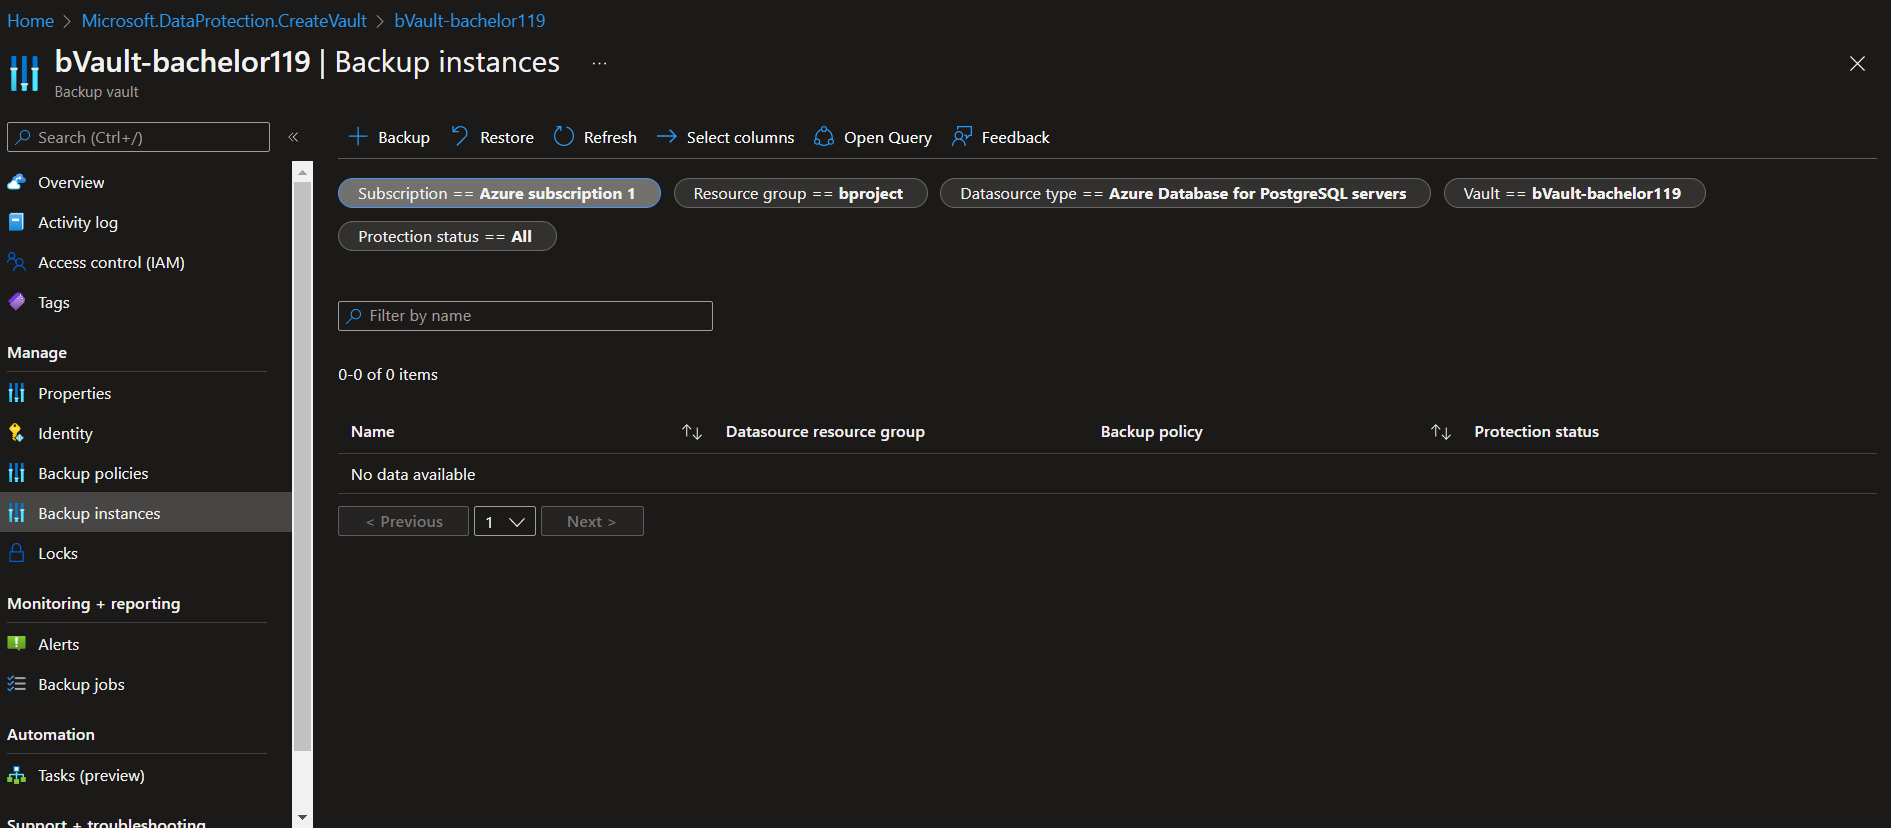
\includegraphics[width=15cm, keepaspectratio]{figures/postgresaasmund/2.PNG}

In the following wizard each organisation must select the options that suit their needs, but importantly it requires the creation of a backup policy. In our example the policy backs up weekly and retains backups for three months. 

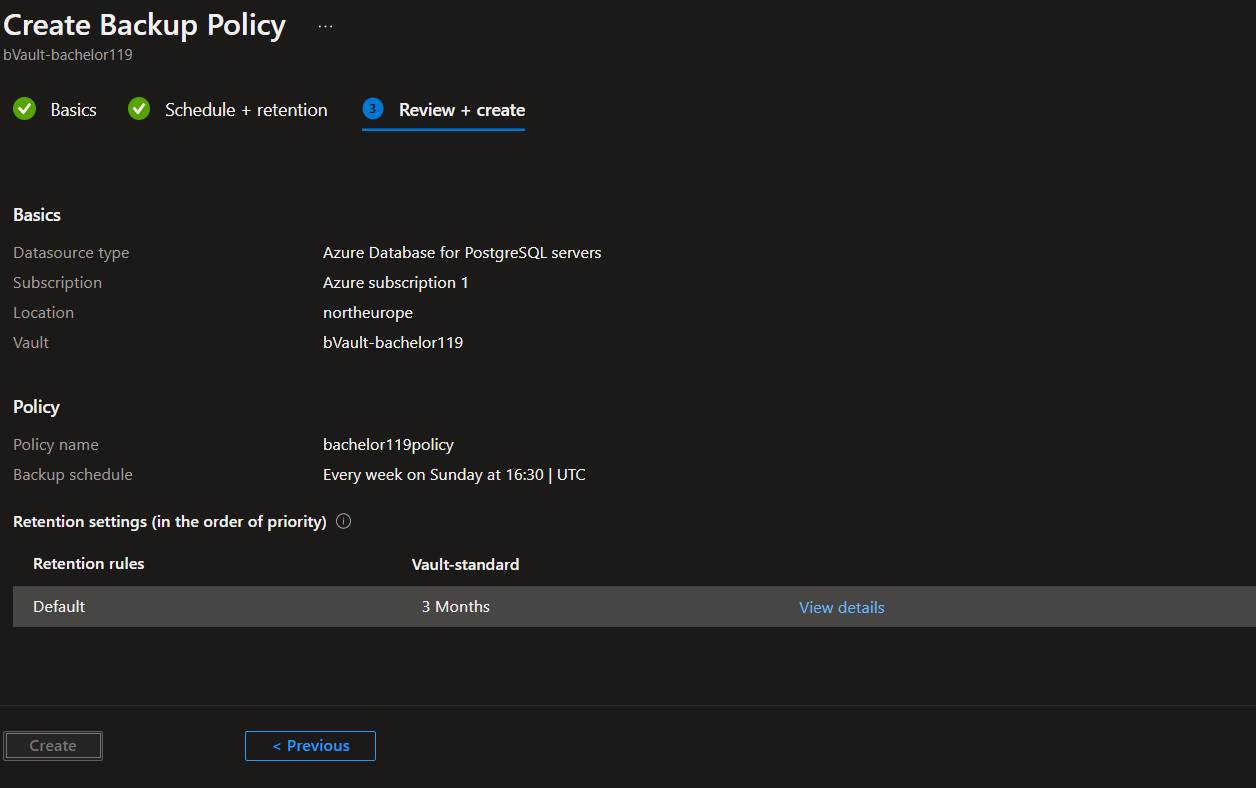
\includegraphics[width=15cm, keepaspectratio]{figures/postgresaasmund/3.PNG}

Additionally when backing up managed postgres servers, we can select which databases to back up. Here we have chosen the standard postgres-database inside the instance, but had we had others we could have chosen them as well. 

When selecting the database we must also give the secret that is required to connect to the database. This can be given as an object i a key vault, as we have done here:

This secret is simply the connection string from the database instance. 

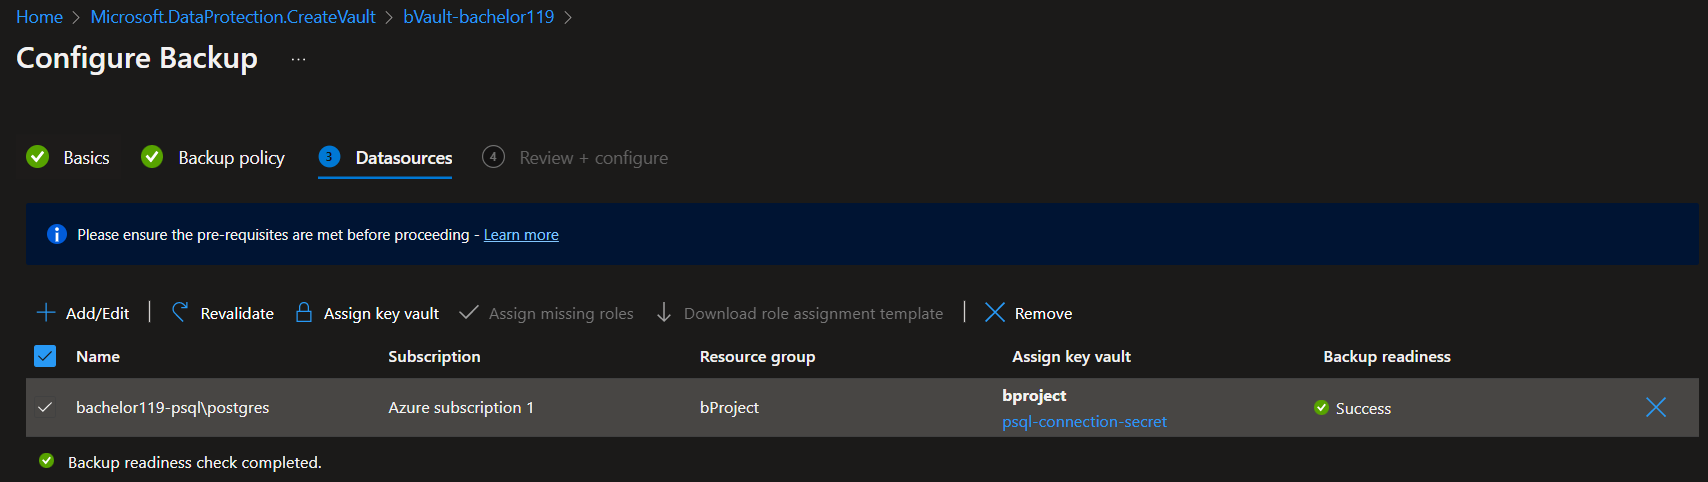
\includegraphics[width=15cm, keepaspectratio]{figures/postgresaasmund/4.PNG}


Finally we have the option to review our options, and if we are happy with these we can create the backup instance. 

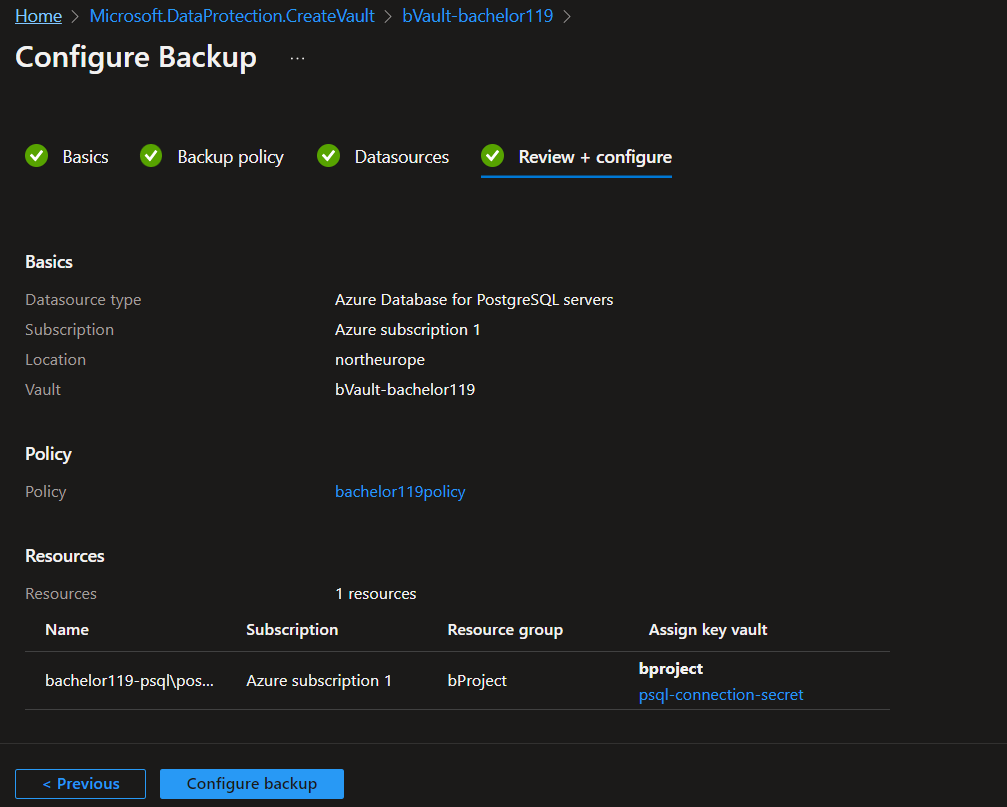
\includegraphics[width=15cm, keepaspectratio]{figures/postgresaasmund/5.PNG}

Immediately after creation the backup instance have not started a backup, and it will not back up the database until we tell it to, or the policy determines that it shall. As shown no backups are completed:

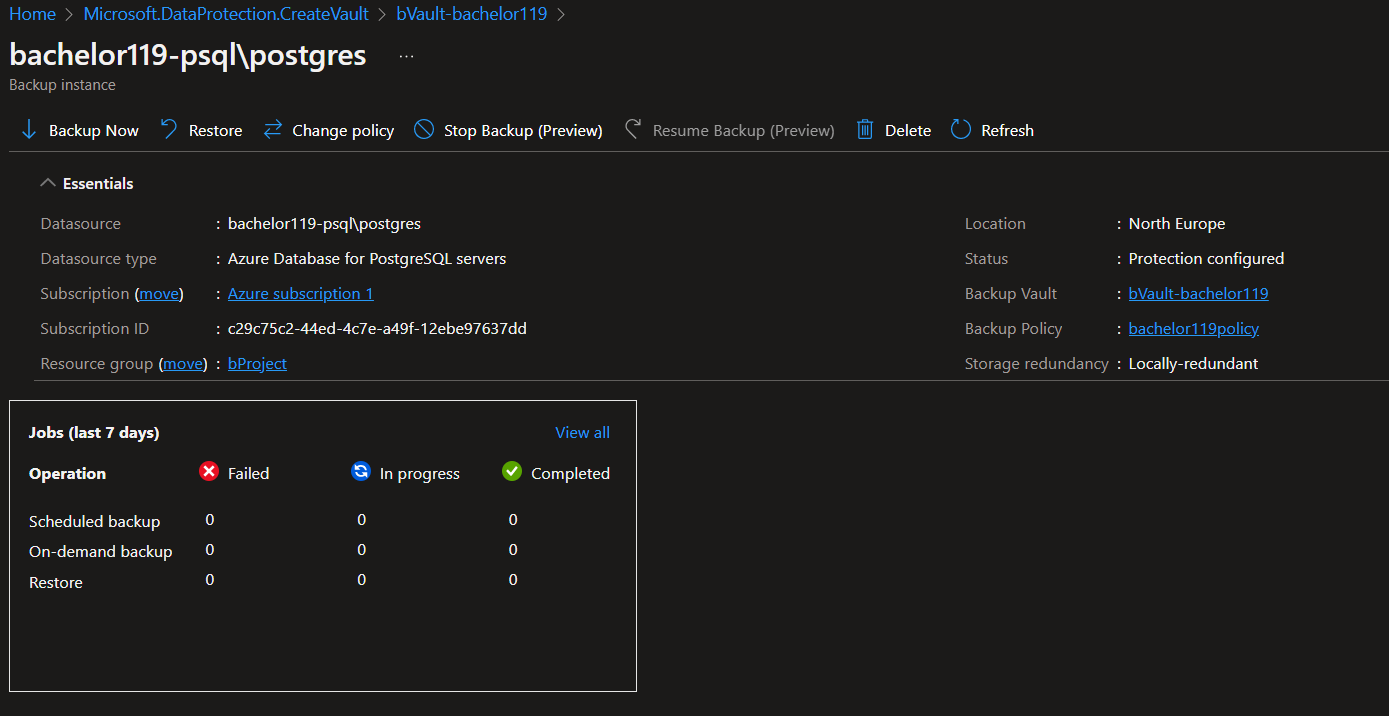
\includegraphics[width=15cm, keepaspectratio]{figures/postgresaasmund/6.PNG}

If we press "back up now" and let it run to completion, we have one completed backup however:

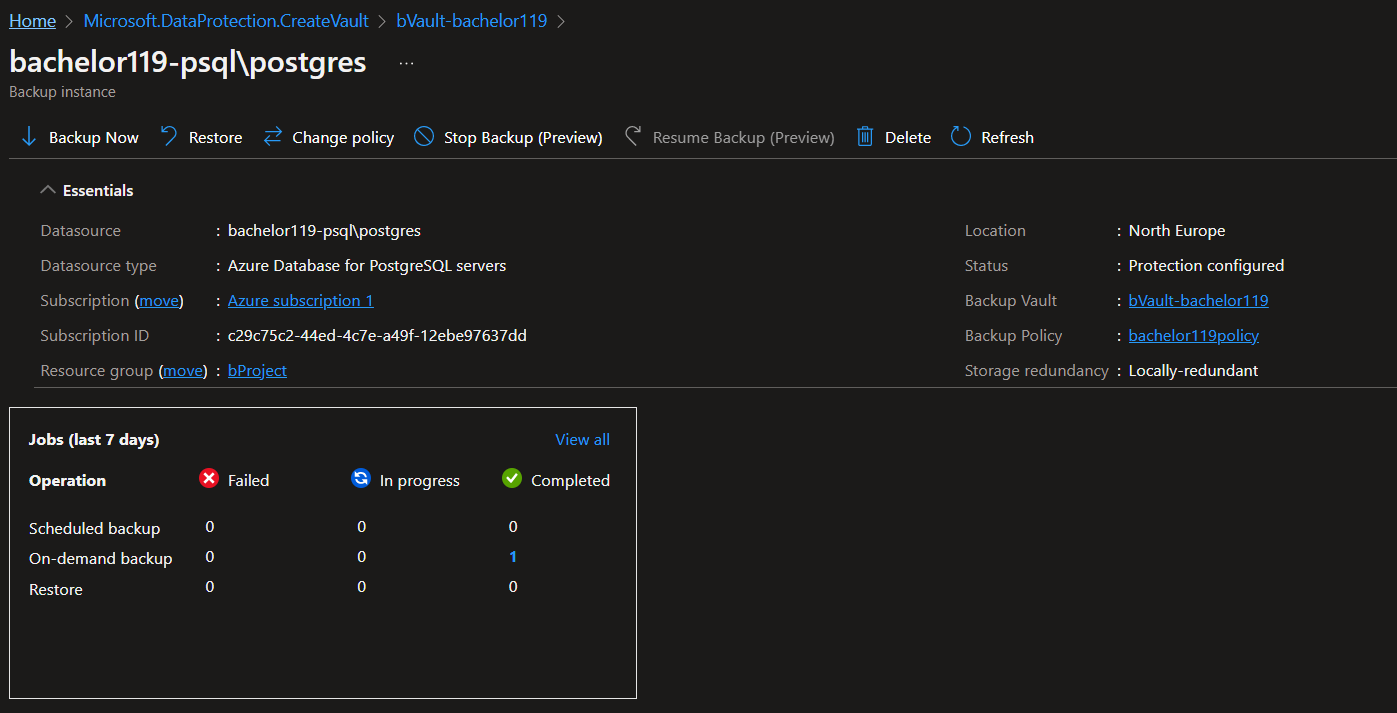
\includegraphics[width=15cm, keepaspectratio]{figures/postgresaasmund/8.PNG}
\label{app_pg_s1e2}